\chapter{背景知識}

\section{HyperText Markup Language(HTML)}\label{s2.1}
\indent
標記式語言(Markup Lanaguage)是一種利用電腦看得懂的標示符號來定義出一份資料會如何呈現在畫面中,
而超文本標記語言(HyperText Markup Language),簡稱HTML,則是用於建立網站的標記式語言,
透過網頁瀏覽器的讀取,可以將其轉換成視覺化的網站。
雖然它不算是程式語言的一種,卻是架構網站的重要根基。

\begin{figure}[H]
    \centering
    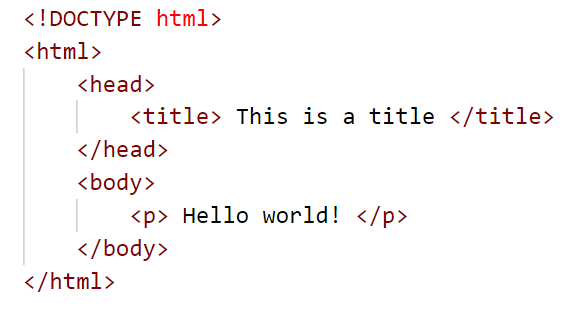
\includegraphics[width=0.55\textwidth]{picture/ch2-htmlExample.png}
    \caption{HTML檔案範例}
    \label{f2.1}
\end{figure}

\section{Node.js}\label{s2.2}
Node.js是一個能夠在伺服器端執行JavaScript的Open Source跨平台執行環境,讓JavaScript這種程式語言不僅僅只能在操作使用者端的程式碼。
它是讓使用者把僅能在瀏覽器執行JavaScript的限制,改成可以透過電腦中的終端介面來直接執行JavaScript程式碼。
而node.js是一個輕量的framework,它裡面的每個JavaScript檔案都會被視為一個module,使用者可以用可下載的或可自己撰寫的模組來實現自己想要的功能。

\subsection{cherrio}\label{s2.2.1}
cherrio是在Node.js的一個模塊,實現了把jQuery中Selector輕量化的功能,需要先讀入HTML進行解析,並使用選擇器找出所需要的元件節點來作客置化的操作。
例如:若需要進行爬蟲的話,需要先讀入一整個完整的網頁HTML,並限制元件的條件來找出該元件來讀出該文字內容。

\subsection{Diff}\label{s2.2.2}
Diff是在Node.js的一個模塊,本論文取用的Hiff開源程式庫是以該模塊為基礎而開發的,利用其中的API來做兩個參數中的比較並顯出是否有差異,參數的類型可以是字元陣列...等等不同類別。

\section{DOM-based Locators}\label{s2.3}
如果要去抓取網頁其中一個物件,並使我們可以透過程式對它進行各式各樣的操作,
方法基本上可以分類成三種:

\indent
1. Coordinate-based locators: 使用座標定位。

\indent
2. DOM(Document Object Model)-based locators: 使用文件物件模型(DOM)定位。

\indent
3. Visual locators: 使用視覺定位,通常使用影像辨識技術。

\indent
本論文中談論的情境是以穩定性較高的DOM-based locators來操作其中的物件,其中DOM在此指的是網頁中的樹狀結構HTML文件結構。
而利用此定位實現的技術即為XPath (XML Path Language)。


\section{XML Path Language (XPath)}\label{s2.4}
XML Path Language (XPath) 是一種用來尋找XML文件中一個或多個節點位置的查詢語言。
以XML中樹狀結構為基礎,讓使用者用一個附帶多個條件的表達式,找到是否有符合這些條件的路徑。

\indent
在Xpath表達式中,最常見的是路徑表達式。
路徑表達式是從一個XML節點到另一個節點或一組節點的步驟順序。
如下圖表示,從HTML起始節點「ul」到屬性id為second-level的節點「li」,再從節點「li」到節點「div」,
其路徑表達式為\colorbox{lightgray}{/ul/li[@id="second-level"]/div}                                                                                                                                                                                                                                                   

\begin{figure}[H]
    \centering
    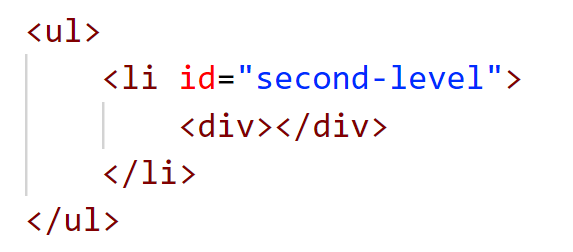
\includegraphics[width=0.5\textwidth]{picture/ch2-xpathExample.png}
    \caption{HTML檔案範例}
    \label{f2.2}
\end{figure}

路徑表達式通常由三個元件設定來組成的,
以圖2.2的路徑表達式為例:

\begin{itemize}
\item[●] 一個 Axis。代表搜尋的方向,例如:路徑表達式中的\colorbox{lightgray}{/}
\item[●] 一個 Node test。可以選擇指定或不指定特定的 HTML 的標籤名稱,例如表達式中的\colorbox{lightgray}{li}
\item[●] 零個或多個 Predicate。描述搜尋節點的條件,藉此可以過濾出需要的節點,例如:\colorbox{lightgray}{/li[@id="second-level"]}
\end{itemize}

% 如圖XXX的HTML結構為例為例,如果需要利用Xpath來定位到[...]的element,將此架構利用這三個元件來一個Xpath表達式。
% \begin{itemize}
%     \item[●] Axis為\colorbox{lightgray}{//},代表搜尋方向為父節點往子節點搜尋,並搜尋所有子孫節點。
%     \item[●] 指定節點名稱為 div 的節點
%     \item[●] 限制該節點有屬性class且屬性值為XXX
% \end{itemize}

% (上述的例子需要補上一張圖)

\section{Chrome Developer tools}\label{s2.5}
基於桌機瀏覽器市占排行,本論文選用市佔率第一個Chrome使用。
在瀏覽器的頁面中,可以點擊功能鍵F12,即可打開它的頁面。
本工具最常用的四個功能模塊為:
\begin{itemize}
    \item[●] 元素(Elements):主要可以展示出該網站的當下HTML檔,以及每個元素對應的CSS屬性...等等細部設定,也可以及時修改當下的檔案,查看若更改會有什麼情況。
    \item[●] 控制台(Console):類似作業系統中的命令提示字元,可以在以網頁的形式讓電腦傳遞給我們一些資訊,例如:輸入Xpath查看是否有定位到該物件以及程式中若需要輸出字元字串,則會在這個頁面下呈現...等等功能。
    \item[●] 源代碼(Sources):從該頁面可以知道該網站的HTML、Javascrpit和CSS...等等程式,也可以從這裡設定斷點,來增加Debug的效率。
    \item[●] 網路(Network):在網站運行時,可以透過該頁面觀察此網頁和伺服器傳遞Request的情況,也可以手動調整網路的速度來檢測網站的穩定性。
\end{itemize}

\begin{figure}[H]
    \centering
    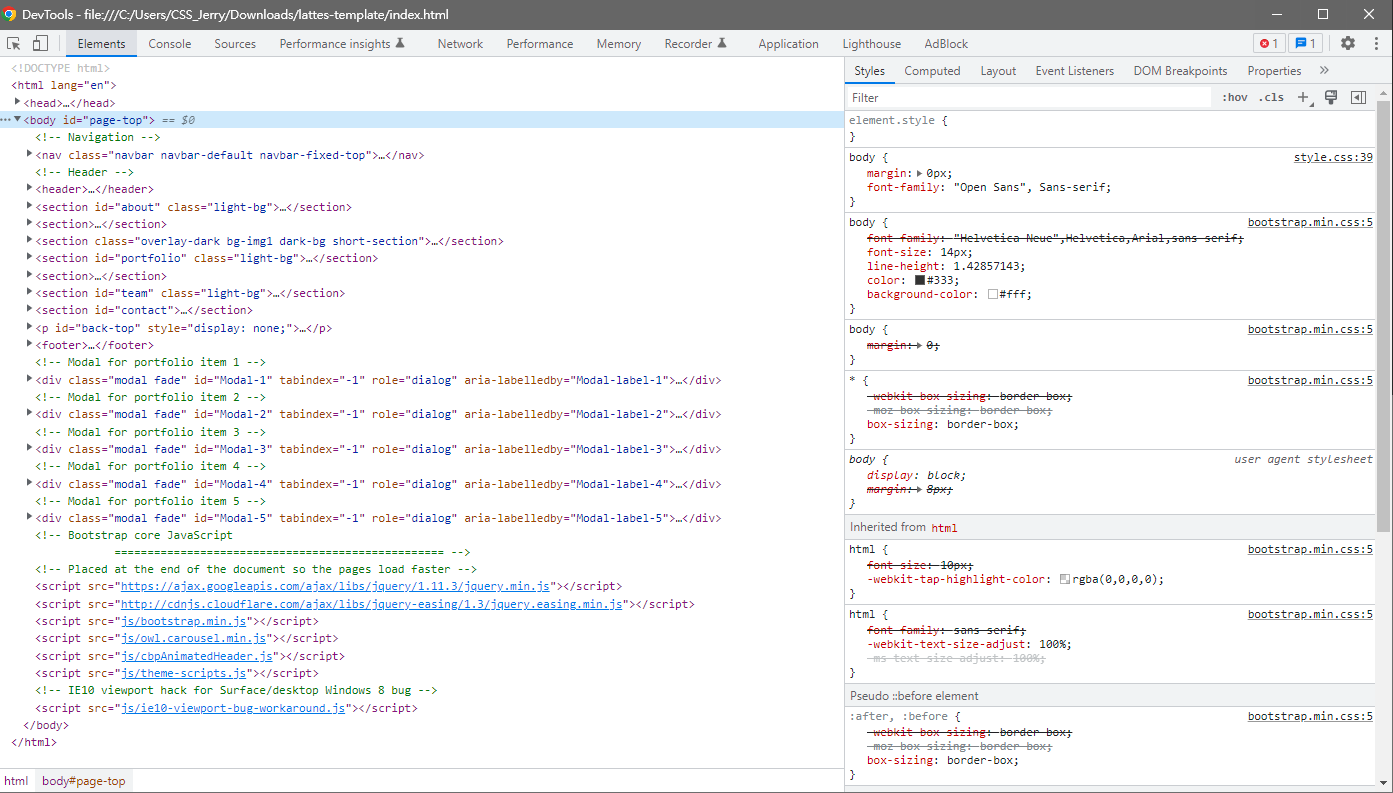
\includegraphics[width=0.8\textwidth]{picture/ch2-chromeDeveloperTool.png}
    \caption{Chrome Developer Tool頁面範例}
    \label{f2.3}
\end{figure}

\section{Chrome Extension}\label{s2.6}

瀏覽器除了有本身基本的功能之外,如果使用者還有其他需求的話,可以去網路商城下載擴充套件或自己撰寫相關程式來讓瀏覽器可以達到使用者額外的需求。
一般來說擴充元件都是用諸如HTML、CSS和JavaScript的網路技術,另外有些還會透過瀏覽器的API來做溝通及變換畫面。
例如:目前市面上有很多人使用網頁版的Google翻譯來解決一般人難以讀懂英文文章的困擾,
但每次都需要跳轉到網頁才可以翻譯,
Google翻譯擴充套件能讓使用者在當下的畫面把文字圈選起來,利用程式判斷出圈起來文字並進行翻譯,
最後在該頁面的HTML增添一些元件來顯示出翻譯的結果供讀者參考。

\subsection{輸入元件}\label{s2.6.1}
Chrome瀏覽器提供能讓使用者和網頁互動的元件,有畫面可見的瀏覽器按鈕和網頁中內容...等等UI元素,也有畫面中的右鍵功能選單和快捷鍵...等等被隱藏的區塊。

\subsection{安裝檔Manifest.josn}\label{s2.6.2}
作為擴充元件的安裝檔,內部記錄了很多很多重要的程式路徑以及權限設定...等等的相關資訊,
若需要將此擴充元件安裝在瀏覽器中使用,需要透過載入此檔案,讓瀏覽器可以支援此程式包的運算邏輯。

\begin{figure}[H]
    \centering
    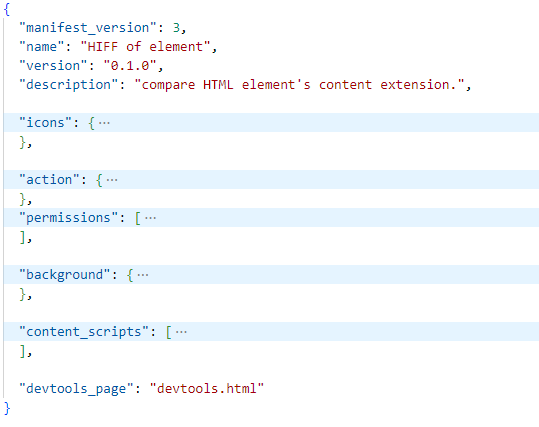
\includegraphics[width=0.6\textwidth]{picture/ch2-manifest.png}
    \caption{Manifest安裝檔範例}
    \label{f2.4}
\end{figure}

\subsection{內部腳本}\label{s2.6.3}
在擴充元件的架構中,根據不同的時機,也有不同的腳本來專門處理同類型的事件,以下列出常用腳本所負責的功能:
\begin{itemize}
    \item[●] Background Script: 一個擴充元件中,專門在背景頁面中執行的腳本,通常是處理程式中的主要邏輯。
    \item[●] Content Script: 在每個網頁頁面(Tab)中,和擴充元件溝通的管道,該腳本會被瀏覽器放入當下頁面的HTML裡面。
    \item[●] Popup Script:瀏覽器中右上角有個擴充元件的頁面按鈕,內部有個獨立的頁面,可以在裡面處理獨立的資訊和畫面。
\end{itemize}
不同的腳本中都有獨立的Scope,可以在內部存儲變數,但它們是不能直接存取對方的資料的,
例如:
Popup Script想要Background Script運算完的結果,
但他們無法互享溝通傳遞變數資料,只能透過Chrome中提供的通訊API,
利用Popup Script告訴Background Script想要你的資料,
Background Script才知道需要運算了並運算結束後結果回傳給Popup.js。

\indent
\begin{figure}[H]
    \centering
    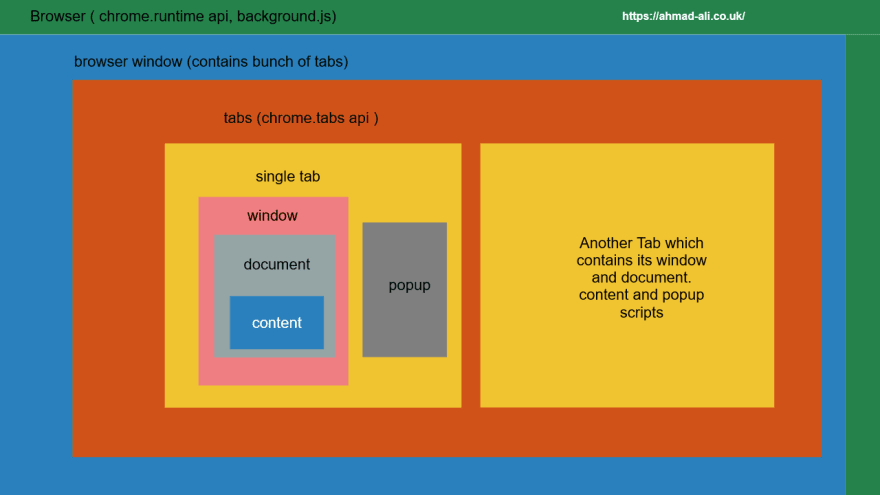
\includegraphics[width=1\textwidth]{picture/ch2-extension-script.png}
    \caption{Manifest安裝檔範例}
    \label{f2.5}
\end{figure}